V této \orig{98} kapitole budeme zkoumat možnosti užití zobecněného
ortogonalizačního algoritmu (kap. 2) k řešení soustav lineárních
algebraických rovnic
%
\begin{align*}
  \tag{11.1}
  Ax + b = 0\Punc{.}
\end{align*}
%
Ukážeme, že je tímto algoritmem možno řešit nejen soustavy se
čtvercovou regulární maticí A, ale i např. soustavy se
singulárními a příp. obdélníkovými maticemi a soustavy homogenní
(b=0). Najdeme rovněž kritéria, podle nichž bude možno
identifikovát soustavy, které nemají řešení. V následujícím textu
budeme předpokládat užití sekvenční varianty algoritmu.
Rozšíření nalezených závěrů i na případ selektivní varianty
algoritmu nečiní obtíží.

\section{Nehomogenní soustava se čtvercovou regulární maticí}

Předpokládejme, že matice \Anxn soustavy (11.1) je
regulární, a že vektor absolutních členů b je nenulový. Probereme
tři různé interpretace soustavy (11.1): dvakrát budeme řešení
soustavy formulovat jako zvláštní případ vyrovnání
zprostředkujících pozorování, jednou jako vyrovnání podmínkových
pozorování. Připomenme, že z uvedených předpokladů vyplývá, že řešení
soustavy (11.1) existuje a je jediné.

\Subsubsection{A} Napišme soustavu rovnic oprav s maticí $A$ a s vektorem
absolutních členů $b$
%
\begin{align*}
  v = Ax + b \Punc{.}
\end{align*}
%
Srovnání (11.1) a (11.2) ukazuje, že lze za uvedených
předpokladů jednoznačně najít hodnoty neznámých tak, aby odpovídající
opravy $v$ byly rovny nule. Řešení soustavy rovnic oprav (11.2)
podle metody nejmenších čtverců vychází z podmínky $(v,v) = \min$.
V daném případě musí tedy vést k neznámým, pro něž je $(v,v)=0$
a tedy i $v=0$. Vzhledem k jednoznačnosti řešení budou neznámé
určené \orig{99} vyrovnáním z (11.2) současně hledanými neznámými,
vyhovujícími soustavě (11.1). Podle kap. 3 mohou být proto
nalezeny zobecněnou ortogonalizací, např. podle schematu

\begin{align*}
\tag{11.3}
\vcenter{\hbox{
  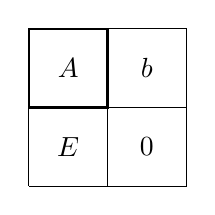
\begin{tikzpicture}[x=1cm,y=1cm]
    \draw (0,1)--(2,1);
    \draw (1,0)--(1,2);
    \draw (0,0) -- (2,0) -- (2,2) -- (0,2) -- (0,0);
    \draw[thick] (0,1) rectangle (1,2);
    \draw (0.5,1.5) node{$A$};
    \draw (1.5,1.5) node{$b$};
    \draw (0.5,0.5) node{$E$};
    \draw (1.5,0.5) node{$0$};
  \end{tikzpicture}
}}
%
\quad\longrightarrow\quad
%
\vcenter{\hbox{
  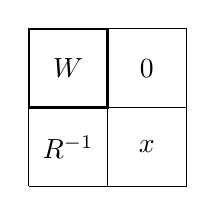
\begin{tikzpicture}[x=1cm,y=1cm]
  \draw (0,1)--(2,1);
  \draw (1,0)--(1,2);
  \draw (0,0) -- (2,0) -- (2,2) -- (0,2) -- (0,0);
  \draw[thick] (0,1) rectangle (1,2);
  \draw (0.5,1.5) node{$W$};
  \draw (1.5,1.5) node{$0$};
  \draw (0.5,0.5) node{$R^{-1}$};
  \draw (1.5,0.5) node{$x$};
\end{tikzpicture}
}}\Punc{.}
\end{align*}


\Subsubsection{B} Uvažujme soustavu podmínkových rovnic s maticí
$A$ a s vektorem absolutních členů $b$
%
\begin{align*}
  \tag{11.4}
  A v + b = 0 \Punc{.}
\end{align*}
%
Z porovnání (11.1) a (11.4) přímo plyne, že opravy jednoznačně
nalezené vyrovnáním podmínkových rovnic (11.4) podle metody
nejmenších čtverců, budou současně řešením soustavy (11.1).
Užijeme-li zobecněné ortogonalizace
%
%
\begin{align*}
\tag{11.3}
\vcenter{\hbox{
  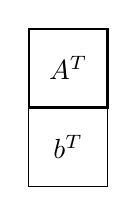
\begin{tikzpicture}[x=1cm,y=1cm]
    \draw[thick] (0,1) rectangle (1,2);
    \draw (0.5,1.5) node{$A^T$};
    \draw (0,0) rectangle (1,1);
    \draw (0.5,0.5) node{$b^T$};
  \end{tikzpicture}
}}
%
\quad\longrightarrow\quad
%
\vcenter{\hbox{
  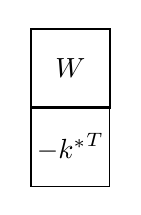
\begin{tikzpicture}[x=1cm,y=1cm]
  \draw[thick] (0,1) rectangle (1,2);
  \draw (0.5,1.5) node{$W$};
  \draw (0,0) rectangle (1,1);
  \draw (0.5,0.5) node{$-{k^\ast}^T$};
\end{tikzpicture}
}}\Punc{.}
\end{align*}
%
%
bude potom v souladu s postupem uvedeným v kap. 3 platit
%
\begin{align*}
  \tag{11.6}
  x = W k^\ast \Punc{.}
\end{align*}


Důležitá přednost formulace B před formulací A spočívá v tom,
že neznámé mohou být nalezeny, aniž by bylo třeba spolu s maticí.
soustavy zpracovávat i jednotkovou matici. Formulace B klade tak
menší nároky na paměť počítače.


\Subsubsection{C} Uvedené dvě
interpretace soustavy lineárních algebraických
rovnic, jednou ve formě soustavy rovnic oprav a po druhé ve
formě soustavy podmínkových rovnic, nejsou jediné. Ukážeme, že lze
najít alternativní převod úlohy na vyrovnání zprostředkujících
pozorování, při němž rovněž nebude nutno zpracovávat jednotkovou
matici. K tomu účelu nejprve dokážeme platnost následující věty.


\vspace{1em}% vertikalni odsazeni stejne jako u subsekci A, B, C ...
\Xemph{Věta 1. Řešíme-li podle metody nejmenších čtverců soustavu
rovnic oprav}
%
\begin{align*}
  \tag{11.7}
  \left[
    \begin{array}{c}
      v_1 \\ v_2
    \end{array}
  \right]
  =
  \left[
    \begin{array}{c}
      A^T \\ b^T
    \end{array}
  \right]
    y
    +
  \left[
    \begin{array}{c}
        0 \\ c
    \end{array}
  \right]\Punc{,} \qquad c \ne 0 \Punc{,}
\end{align*}
%
\Xemph{pak \orig{100} pro řešení soustavy (11.1) platí}
%
\begin{align*}
  \tag{11.8}
  x = {1\over{v_2}} \;v_1 \Punc{.}
\end{align*}
%


\Xemph{Důkaz}. V práci [22] jsou mj. odvozeny vzorce umožňující
najít opravy ve vyrovnávací úloze, která vznikla z některé
výchozí úlohy připojením dalších rovnic oprav. V našem případě je
výchozí úloha definována rovnicí
%
\begin{align*}
  \tag{11.9}
  v_1^{(0)} = A^T y^{(0)} + 0
\end{align*}
%
s triviálním řešením $v_1^{(0)} = 0$, $y^{(0)} = 0$. Označíme-li
%
\begin{align*}
  \tag{11.10}
  \beta = \big(AA^T\big)^{-1} b \Punc{,}
\end{align*}
%
pak podle [22], s užitím naší symboliky a s uvážením
předpokladu o regularitě matice $A$, bude
%
\begin{align*} % predpoklad: A je regularni
  \tag{11.11}
  v_1 &= v_1^{(0)} - v_2 A^T\beta = v_2 A^T \big(AA^T\big)^{-1}b = v_2 x \\
  \tag{11.12}
  v_2 &= {{b^T y^{(0)} + c}\over{1 + b^T\beta}}
       =  {c\over{1+ b^TA^{-T}A^{-1}}b} = {c\over{1 + x'x}} \ne 0.
\end{align*}
%
Uvážíme-li platnost (11.12), plyne dokazovaný vztah (11.8)
bezprostředně z (11.11).

Věta 1 umožňuje podle (11.8) vypočítat neznámé v soustavě
(11.1) prostřednictvím oprav náhradní úlohy (11.7). Užijeme-li
k nalezení těchto oprav zobecněné ortogonalizace
\begin{align*}
  \tag{11.13}
  \vcenter{\hbox{
  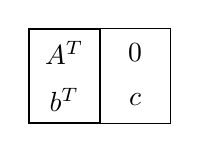
\begin{tikzpicture}[xscale=0.9,yscale=0.6]
  \draw[thick] (0,0) rectangle (1,2);
  \draw (0.5,1.5) node{$A^T$};
  \draw (0.5,0.5) node{$b^T$};
  \draw (1,0) rectangle (2,2);
  \draw (1.5,1.5) node{$0$};
  \draw (1.5,0.5) node{$c$};
  \end{tikzpicture}}}
  %
  \quad\longrightarrow\quad
  %
  \vcenter{\hbox{
  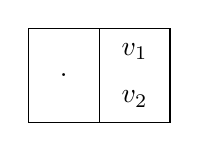
\begin{tikzpicture}[xscale=0.9,yscale=0.6]
  \draw (0,0) rectangle (1,2);
  \draw (0.5,1) node{$.$};
  %\draw (0.5,0.5) node{$b^T$};
  \draw (1,0) rectangle (2,2);
  \draw (1.5,1.5) node{$v_1$};
  \draw (1.5,0.5) node{$v_2$};
  \end{tikzpicture}}}
  \Punc{,}
\end{align*}
%
pak není třeba určovat neznámé $y$ a není tedy ani třeba zpracovávat
jednotkovou \orig{101} matici.%
%
\footnote{
K numericky ekvivalentnímu algoritmu dochází odlišným
způsobem \name{VOJEVODIN} [41, str. 84]; viz též [24], procedura OR.}
%
Formulace (C) na rozdíl od (A) a (B)není zřejmě vhodná pro současné
řešení většího počtu soustav rovnic, které se liší pouze vektory svých
absolutních členů.


\section{Homogenní soustava}

Hledejme nyní ortogonalizačním algoritmem netriviální řešení
homogenní soustavy $m$ rovnic o $n$ neznámých
%
\begin{align*}
  \tag{11.14}
  A x = 0 \Punc{.}
\end{align*}
%
Sloupce matice \Amxn označme $a_i$ $(i=1,2,\ldots,n)$, její hodnost
nechť je $h$.

Všechna řešení soustavy (11.14) tvoří, jak známo [37, str. 82],
vektorový prostor dimenze $k=n-h$. Kdybychom znali libovolnou bázi
tohoto prostoru, tzv.  \Xemph{fundamentální soustavu řešení}
%
\begin{align*}
  \tag{11.15}
  \left\{\; x^{(1)}, x^{(2)}, \ldots, x^{(k)\;}\right\} \Punc{,}
\end{align*}
%
potom každé řešení soustavy (11.14) můžeme vyjádřit jako
lineární kombinaci
%
\begin{align*}
  \tag{11.16}
  x = \sum_{i=1}^k \alpha_i x^{(i)} \Punc{,}
\end{align*}
%
kde $\alpha_i$ jsou libovolné konstanty.


Naší snahou bude ukázat, jak může být fundamentální soustava
řešení (11.15) nalezena zobecněným ortogonalizačním algoritmem.
V dalším budeme uvažovat pouze variantu A řešení soustav rovnic,
popsanou v odst. 11.1, tj. budeme užívat zobecněné
ortogonalizace podle (11.3) s nulovým vektorem absolutních členů.

Předpokláde jme nejprve, že všechny sloupce matice $A$ jsou
lineárně nezávislé. Pak ovšem $h=n$, prostor řešení má dimenzi $k=0$
a existuje pouze triviální řešení $x=0$ soustavy (11.14). Toto
řešení bude bezprostředně nalezeno ortogonalizačním algoritmem.

Nechť \orig{102} nyní hodnost matice $A$ je menší než počet jejích
sloupců. Potom existuje matice $A_1$ $(m \times h)$, tvořená lineárně
nezávislými sloupci matice $A$ a matice $A_2$ $(m \times k)$, jejíž
sloupce lze vyjádřit jako lineární kombinace sloupců matice
$A_1$. Sloupce matice $A_2$ označme $a_i^N$ $(i=1,2,\ldots,h)$,
sloupce matice $A_2$ budou $a_j^Z$ $(j=1,2,\ldots,k)$. Platí
%
\begin{align*}
  \tag{11.17}
  a_j^Z = c_{1j}a_1^N + c_{2j}a_2^N + \ldots + c_{hj}a_h^N, \qquad
          (j=1,2,\ldots,h) \Punc{,}
\end{align*}
%
kde konstanty $c_{ij}$ představují koeficienty zmíněné lineární
kombinace. Zavedeme-li matici $C = \Vert c_{ij} \Vert \;\; (h \times k)$,
pak platí
\begin{align*}
  \tag{11.18}
  A_2 = A_1C \Punc{.}
\end{align*}
%
Označme $x_1$ neznámé odpovídající vybraným lineárně nezávislým
sloupcům matice $A$ a $x_2$ neznámé odpovídající zbývajícím sloupcům.
Potom bude
%
\begin{align*}
  \tag{11.19}
  Ax = A_1x_1 + A_2x_2 = A_1x_1 + A_1Cx_2 = A_1(x_1 + Cx_2)
\end{align*}
%
a podle (11.14)
%
\begin{align*}
  \tag{11.20}
  A_1(x_1 + Cx_2) = 0 \Punc{.}
\end{align*}
%
Soustava (11.20) představuje homogenní soustavu s maticí, jejíž
sloupce jsou lineárně nezávislé, a která má proto pouze
triviální řešení
\begin{align*}
  \tag{11.21}
  x_1 + Cx_2 = 0 \Punc{.}
\end{align*}
%

Pro zjednodušení symboliky budeme dále bez omezení obecnosti
našich závěrů předpokládat, že vektor $x_1$ je tvořen prvními $h$
neznámými; první $h$ sloupce matice $A$ jsou tedy lineárně nezávislé.
Potom každý vektor
%
\begin{align*}
  \tag{11.22}
  x = \left[
    \begin{array}{c}
      x_1 \\ x_2
    \end{array} \right] \Punc{,}
\end{align*}
%
jehož složky $x_1$ a $x_2$ vyhovují rovnici (11.21) bude, jak se
snadno přesvědčíme dosazením do (11.19), hledaným řešením soustavy
(11.14). Chceme-li najít fundamentální soustavu řešení (11.15),
stačí nyní určit $k$ lineárně nezávislých vektorů $x^{(i)\!}$, vyhovujících
%
(11.21). Označme \orig{103} v~souladu s (11.22)
%
\begin{align*}
  \tag{11.23}
  X = \left[
    \begin{array}{c}
      X_1 \\ X_2
    \end{array} \right] =
  \left[
    \begin{array}{cccc}
      x_1^{(1)} & x_1^{(2)} & \ldots & x_1^{(k)}  \\
      x_2^{(1)} & x_2^{(2)} & \ldots & x_2^{(k)}  \\
    \end{array} \right]
\end{align*}
%
matici typu $(n \times k)$ tvořenou hledanými vektory. Položíme-li
potom
%
\begin{align*}
  \tag{11.24}   X_2 &= E\quad (k \times k) \\
  \tag{11.25}   X_1 &= -C X_2 = -C \Punc{,}
\end{align*}
%
budou sloupce odpovídající matice $X$ zřejmě tvořit fundamentální
soustavu řešení systému (11.14). V důsledku (11.24) jsou
totiž tyto sloupce lineárně nezávislé a jejich složky vyhovují
podle (11.25) rovnici (11.21). Fundamentální soustava řešení,
definovaná rovnicemi (11.24) a (11.25) bývá někdy označována jako
normální [37, str. 82].

Souhrnně můžeme konstatovat, že pro vyřešení dané úlohy v podstatě
stačí najít prvky matice $C$, tj. podle (11.17) koeficienty lineárních
kombinací $h$ nezávislých sloupců matice $A$, vyjadřujících
zbývajících $k$ lineárně závislých sloupců této matice.  V odst. 8.1
jsme ukázali, že existence lineárně závislého sloupce v matici $A$ se
projevuje jako tzv. singularita prvního druhu.  Hledané koeficienty
lze v takových případech určit podle (8.10) dělením naddiagonálních
prvků matice $R^{-1}$ prvky diagonálními v těch slouncích horní
trojúhelníkové matice $R^{-1}$ (11.3), které odpovídají lineárně
závislým sloupcům matice $A$.

Při užití procedury ORTON3 k řešení homogenní soustavy rovnic
dochází po zjištění singularity prvního druhu např. u s-tého
sloupce matice $A$ k tisku prvků s-tého sloupce matice
$R^{-1}$ formou
%
% LIN. DEP. COL. NO. 5
% m+1   r15
% m+1   r15
% \vdots
% m+1   r15
\begin{align*}
  \tag{11.26}
  \begin{array}{cl}
  \multicolumn{2}{l}{\small\texttt{LIN. DEP. COL. NO. 5}} \\
  m+1 & r_{15} \\
  m+2 & r_{25} \\
  \vdots & ~~\vdots \\
  m+n & r_{n5}\Punc{,} \\
  \end{array}
\end{align*}
%
kde \orig{104} $r_{is}$ značí prvek v i-tém řádku s-tého sloupce matice
$R^{-1}$.%
\footnote{
Prvky $r_{is}$  jsou po vytištění nulovány, jak jsme viděli v
odst. 8.1.
}
%
Porovnáním (8.10),(11.24) a (11.25) snadno ověříme, že pro
složky odpovídajícího vektoru normální fundamentální soustavy
(např. $x^{(t)}$) platí
%
\begin{align*}
  \tag{11.27}
  x^{(t)} = r_{is}/r_{ss} \Punc{,} \quad(i=1,2,\ldots,n) \Punc{.}
\end{align*}

Soustava (11.14), při jejímž řešení nedojde k tisku (11.26),
bude mít pouze triviální řešení $x=0$.

~

\noindent
\Xemph{Numerický příklad [37, str. 89, příklad 8]}

~

Hledáme normální fundamentální soustavu řešení systému rovnic
%
\begin{align*}
  x_1 + x_2 + x_3 + x_4 + x_5 &= 0 \\
  3x_1 + 2x_2 + x3 + x_4 - 3x_5 & = 0 \tag{11.28} \\
  x_2 + 2x_3 + 2x_4 + 6x_5 &= 0 \\
  5x_1 + 4x_2 + 3x_3 + 3x_4 - x_5 &= 0 %\Punc{.}
\end{align*}
%
Je tedy $m=4$ a $n=5$. Při výpočtu úlohy podle programu
ORTON3-ZKOUŠKA1 (kap. 13) se ukázalo podle tisků
%
\begin{align*}
  \newcolumntype{T}{>{\ttfamily\normalsize}c}
  \newcommand{\X}[2]{#1_{10}#2}% Elliot float number style
  %\newcommand{\X}[2]{#1\texttt{e}#2}% usual float number style
  \tag{11.29}
  \begin{array}{lrlrlr}
    \multicolumn{2}{r}{\small\texttt{LIN.DEP.COL.NO.3~}} &
    \multicolumn{2}{r}{\small\texttt{LIN.DEP.COL.NO.4~}} &
    \multicolumn{2}{r}{\small\texttt{LIN.DEP.COL.NO.5~}} \\
    5 & \X{~3.33333327}{-01} & 5 & \X{~3.33333327}{-01} & 5 & \X{~8.33333331}{-01} \\
    6 & \X{-6.66666659}{-01} & 6 & \X{-6.66666659}{-01} & 6 & \X{-9.99999995}{-01} \\
    7 & \X{~3.33333333}{-01} & 7 & \X{~0.00000000}{+00} & 7 & \X{~0.00000000}{+00} \\
    8 & \X{~0.00000000}{+00} & 8 & \X{~3.33333333}{-01} & 8 & \X{~0.00000000}{+00} \\
    9 & \X{~0.00000000}{+00} & 9 & \X{~0.00000000}{+00} & 9 & \X{~1.66666667}{-01} \\
  \end{array}  %\Punc{,}
\end{align*}

\noindent
že tři poslední sloupce v matici soustavy (11.28) jsou
lineárně závislé na jejích prvních dvou sloupcích. Prostor řešení má
tedy dimenzi $k=3$. Jak je patrno z (11.29), můžeme za bázi
tohoto prostoru považovat vektory
%
\orig{105}
\begin{align*}
  \tag{11.30}
  \begin{array}{ccccccc}
  x^{(1)} = (& 1/3 & -2/3 & 1/3 &  0  &  0  &)^T, \\
  x^{(2)} = (& 1/3 & -2/3 &  0  & 1/3 &  0  &)^T, \\
  x^{(3)} = (& 5/6 &  -1  &  0  &  0  & 1/6 &)^T.
  \end{array}
\end{align*}
%
Podle (11.27) je příslušná normální fundamentální soustava
%
\begin{align*}
  \tag{11.31}
  \begin{array}{ccccccc}
  x^{(1)} = (&  1  &  -2  &  1  &  0  &  0  &)^T, \\
  x^{(2)} = (&  1  &  -2  &  0  &  1  &  0  &)^T, \\
  x^{(3)} = (&  5  &  -6  &  0  &  0  &  1  &)^T.
  \end{array}
\end{align*}
%
Uvedený příklad, stejně jako příklad v následujícím odstavci,
má pouze ilustrativní charakter. Je samozřejmé, že zkušený
počtář by v praxi takové úlohy neřešil na počítači, ale
jednoduchým úsudkem.

\section{Nehomogenní soustava s obecnou maticí}

Obraťme svou pozornost ještě na řešení soustav s obecnou
maticí \Amxn a nenulovým vektorem absolutních členů $b$. Matice
soustavy může tedy být např. obdélníková nebo čtvercová
singulární. Podle \name{KRONECKEROVY} věty [37, str. 78] je taková soustava
řešitelná právě tehdy, je-li hodnost $h$ matice $A$ rovna hodnosti
$h_r$, matice rozšířené $[A b]$. Řešení, pokud existuje, nemusí
být jednoznačné. Je známo [37, str. 83], že obecné řešení
soustavy (11.1) lze vyjádřit jako součet
%
\begin{align*}
  \tag{11.32}
  x = x_0 + y \Punc{,}
\end{align*}
%
kde $x_0$ je libovolné pevně zvolené řešení soustavy (11.1) a $y$
probíhá prostor řešení homogenní soustavy s touž maticí $A$.
Chápáno geometricky, vytvářejí všechna řešení soustavy (11.1)
nadrovinu dimenze $(n-h)$.

V minulém odstavci jsme ukázali, jak lze ortogonalizačním
algoritmem najít obecné řešení homogenní soustavy. Abychom mohli
%
vyjádřit \orig{106} všechna řešení nehomogenní soustavy (11.1), stačí
tedy Ještě najít jediné konkrétní řešení X- této soustavy.
V dalším ukážeme, jak může být takové řešení nalezeno
ortogonalizačním algoritmem (konkrétně procedurou ORTON3 - kap. 12)
a jaké má bližší vlastnosti, Dokud má soustava řešení více. Stejně
jako v odst. (11.1) probereme opět tři postupy A, B a C. U každého
z nich uvedeme kritérium, podle něhož je možno rozlišit, zda
předložená soustava má nebo nemá řešení. U neřešitelných
soustav se u formulací A a B ukáže, že ortogonalizační algoritmus
poskytuje určité \uv{náhradní} hodnoty neznámých, jejichž
vlastnosti rovněž vyšetříme.

\Subsubsection{A} Řešení přechodem na soustavu rovnic oprav (11.2)

\Subsubsection{A.1}  Úloha je řešitelná

Stejnou úvahou jako v odst. 11.1 dospějeme k závěru, že
zobecněným ortogonalizačním algoritmem budou podle (11.3)
nalezeny neznámé, pro něž je $v=O$, tedy neznámé vyhovující soustavě
(11.1). V případě soustavy, která není řešitelná jednoznačně,
bude nalezeno to řešení, v němž neznámé, odpovídající lineárně
závislým sloupcům, budou rovny nule. Toto konstatování
bezprostředně vyplývá z postupu užívaného procedurou ORTON3 při
zjištění singularity prvního druhu (odst. 8.1).

\Subsubsection{A.2}  Úloha je neřešitelná

V takovém případě musí být vektor $v$ nenulový (příznak
neřešitelnosti). Úloha se řeší jako vyrovnání zprostředkujících
pozorování, takže bude nalezeno náhradní řešení, vyznačující se
minimální délkou reziduového vektoru. Pokud je $h< n$, budou stejně
jako ad A.1 hodnoty neznámých, odpovídajících lineárně závislým
sloupcům, rovny nule.


\Subsubsection{B} Řešení přechodem na soustavu podmínkových rovnic (11.4)

\Subsubsection{B.1} Úloha je řešitelná

Ortogonalizačním algoritmem bude podle (11.5) a (11.6)
nalezeno řešení, vyhovující soustavě (11.1). Pokud existuje větší
počet řešení, bude nalezen vektor neznámých s minimální délkou.
%
Hodnoty \orig{107} neznámých budou obecně jiné, než v případě A.1.

\Subsubsection{B.2} Úloha je neřešitelná

Úloha bude řešena jako vyrovnání podmínkových pozorování,
kde lineárně závislé řádky matice $A$ a jim odpovídající
absolutní členy byly vypuštěny (odst. 8.2), Bude tak nalezeno
řešení těch rovnic soustavy (11.1), které si neodporují. Je-li
takových řešení více, bude, stejně jako v odst. B.l, nalezen
vektor neznámých s minimální délkou. Rovnice,jimž nebylo
vyhověno, je třeba hledat mezi těmi, které odpovídají
vypuštěným řádkům matice $A$. Jsou to ty z nich, pro něž je odpovídající
nodnota $k_i^*$ (odst. 8.2) nenulová (příznak neřešitelnosti).
Vypuštění rovnice je procedurou ORTON3 signalizováno v analogii
k (11.26) tiskem
%
\begin{align*}
  \tag{11.33}
    \begin{array}{cl}
  \multicolumn{2}{l}{\small\texttt{LIN. DEP. COL. NO. $i$}} \\
  n+1 & -k_i^*\Punc{.} \\
  \end{array}
\end{align*}

Postupem naznačeným v odst. 8.2 lze při formulaci B najít
numerické hodnoty koeficientů, pomocí nichž je možno vyjádřit
lineárně závislé řádky matice $A$ jako lineární kombinace
předchozích nezávislých řádků. Tento postup ovšem předpokládá, že
spolu s maticí A byla ortogonalizačním algoritmem zpracována i
jednotková matice.




\Subsubsection{C} Řešení přechodem na soustavu rovnic oprav (11.7)

\Subsubsection{C.1} Úloha je řešitelná

Uvažujme soustavu rovnic oprav (11.7), kde $A^T$ nyní bude
obecná matice typu $(n \times m)$, příslušná řešené soustavě (11.1).
Hodnost matice soustavy (11.7) nechť je $h_r$ $(\le m)$. Z kap. 3 víme,
že zobecněný ortogonalizační algoritmus bude v takovém případě
operovat s $h_r$, lineárně nezávislými sloupci této matice.
Ostatní sloupce budou ignorovány. Označíme-li $[A_1 b_1]$ matici
tvořenou lineárně nezávislými řádky natice $[A b]$ (11.1), pak
řešení soustavy (11.7) ortogonalizačním algoritmen zřejmě
přejde na řešení úlohy
%
\orig{108}
\begin{align*}
  \tag{11.34}
  \left[
    \begin{array}{c}
      v_1 \\ v_2
    \end{array}\right] =
  \left[
    \begin{array}{c}
      A_1^T \\ b_1^T
    \end{array}\right] y_1 +
  \left[
    \begin{array}{c}
      0 \\ c
    \end{array}\right]\Punc{,} \qquad c \ne 0 \Punc{.}
\end{align*}
%
Najdeme vztah mezi hledanými neznámými, které vyhovují
soustavě (11.1) a opravami $v_1$ a $v_2$ úlohy (11.34).

Matice soustavy (11.34) má lineárně nezávislé sloupce. Lze
snadno dokázat, že rovněž sloupce matice $A^T$ musí být lineárně
nezávislé. Aplikací vzorců (11.11) a (11.12) potom dostaneme
%
\begin{align*}
  \tag{11.35}
  v_1 = -v_2A_1^T \big(A_1A_1^T\big)^{-1} b_1, \qquad
  v_2 = {c\over1+b_1^T \big(A_1A_1^T\big)^{-1} b_1} \Punc{.}
\end{align*}
%
Matice $A_1$ obecně nemá inverzní matici, nemůžeme tedy při úpravě
(11.35) užít postupu, který sloužil k úpravě (11.11) a (11.12),
Vyjdeme proto z následující úvahy. Soustava rovnic
%
\begin{align*}
  \tag{11.36}
  A_1x + b_1 = 0
\end{align*}
%
je zřejmě řešitelná. Jedno řešení může být nalezeno např. tak,
že soustavu (11.36) považujeme za soustavu podmínkových rovnic
a řešíme podle metody nejmenších čtverců. Najdeme tak vektor $x_e$,
který má nejmenší délku ze všech vektorů, vyhovujících (11.36)
a tedy i (11.1). Podle vzorců pro vyrovnání podmínkových
pozorování platí (viz odst. 3.2)
%
\begin{align*}
  \tag{11.37}
  x_e = -A_1^T \big(A_1A_1^T\big)^{-1} b_1, \qquad
  (x_e,x_e) = b_1^T \big(A_1A_1^T\big)^{-1} b_1 \Punc{.}
\end{align*}
%
Vraťme se nyní ke vzorci (11,35), který můžeme s využitím (11.37)
psát ve tvaru
\begin{align*}
  \tag{11.38}
  v_1 = v_2 x_e\Punc{,} &\qquad v_2 = {c\over 1 + (x_e,x_e)}
  \quad \ne 0\Punc{,}
  \shortintertext{takže}
  \tag{11.39}
  x_e &= {1\over v_2} v_1 \Punc{.}
\end{align*}
%
Docházíme tedy k tomuto závěru: Užijeme-li pro řešení soustavy
formulace C, potom za předpokladu, že řešení existuje, vede
%
\orig{109} ortogonalizační elgoritmus prostřednictvím (11.39) k
neznámým s minimální euklidovskou normou. Formulace C dává tedy v
takovém případě stejné výsledky jako formulace B.

\Xemph{Poznámka}. Z uvedeného rozboru vyplývá mj. zajímavý závěr o
jejné obecné možnosti převodu vyrovnání podmínkových pozorování
na vyrovnání zprostředkujících pozorování. Opravy vyhovující
podmínkovým rovnicím (11.36) lze totiž najít ze vzorce (11.39)
pomocí oprav $v_1$ a $v_2$, určených vyřovnáním (11.34) podle
zprostředkujících pozorování.

\Subsubsection{C.2}Úloha je neřešitelná

Budeme zkoumat vlestnosti oprav $v_1$ a $v_2$, získaných řešením
soustavy (11.7) zobecněným ortogonalizačním alzoritmem.
Předpokládáme, že korespondující soustava (11.1) nemá řešení,
takže pro hodnost $h$ matice $A$ a hodnost $h_r$, matice
$[A~b]$ platí nerovnost
%
\begin{align*}
  \tag{11.40}   h_2 > h \Punc{.}
\end{align*}
%


Nejprve dokážeme, že v rovnicích (11.7) je možno najít vektor $y$ tak,
aby odpovídající opravy $v_1$ a $v_2$ byly nulové. Chceme tedy
prokázat řešitelnost soustavy rovnic
%
\begin{align*}
  \tag{11.41}
  \begin{array}{lll}
  A^Ty     & =& 0 \\
  b^Ty + c & =& 0 \Punc{.}
  \end{array}
\end{align*}
%
Označme $A_1^T$ matici tvořenou $h$ lineárně nezávislými řádky matice
$A^T$. Najdeme-li řešení soustavy rovnic
%
\begin{align*}
  \tag{11.42}
  \begin{array}{lll}
  A_1^Ty   & =& 0 \\
  b^Ty + c & =& 0 \Punc{,}
  \end{array}
\end{align*}
%
pak jsme zřejmě našli i řešení rovnic (11.41). Prověříme, zda
je splněna nutná a postačující podmínka řešitelnosti soustavy
(11.42), totiž zda hodnost matice
%
$ S = \left[\begin{array}{c}A_1^T \\ b^T \end{array} \right] $
%
je rovna hodnosti rozšířené matice \orig{110}
%
$
S_r = \left[
  \begin{array}{cc}
    A_1^T & 0 \\ b^T & c
  \end{array}
  \right]
$.
%
Hodnost matice $A$ je rovna $h$.  V důsledku (11.40) je vektor $b$
lineárně nezávislý na sloupcích matice $A$, takže i vektor $b^T$ je
lineárně nezávislý na řádcích matice $A^T$ a tedy i $A_1^T$. Hodnost
matice $S$ musí proto být rovna $(h+1)$.  Obraťme se nyní k matici
$S_r$. Počet řádků matice $S_r$ je roven $(h+1)$.  Hodnost matice
$S_r$ nemůže být větší než počet řádků a tudíž je menší nebo rovna
$(h+1)$.  Na druhé straně hodnost rozšířené matice $S_r$ nemůže být
menší než hodnost matice $S$.  Hodnost matice $S_r$ je tedy právě
rovna $(h+1)$ a je proto stejná jako hodnost matice $S$. Dokázali jsme
tedy, že soustava (11. 42) stejně jako soustava (11.41) jsou
řešitelné, tekže vektor $y$ anulující opravy v soustavě rovnic oprav
(11.7) existuje.

Řešením soustavy rovnic oprav (11.7) podle metody nejmenších
čtverců hledáme takové hodnoty neznámých, pro něž je $(v,v)$
minimální. V daném případě je však, jak jsme právě dokázali,
možno dosáhnout $(v,v) = 0$, Ortogonalizační algoritmus, o němž z
kan. 8 víme,že najde řešení i v případě, že matice soustavy
rovnic oprav obsahuje lineárně závislé sloupce, Dovede tedy k
nulovým opravám.


Ukázali jsme, že při užití formulace C bude neřešitelnost
soustavy (11.1) signalizována nulovými hodnotami oprav $v_1$ a $v_2$.
Na rozdíl od formulací A a B nebude v takovém případě nalezeno
žádné náhradní řešení.

~

\noindent
\Xemph{Numerický příklad [37, str. 89, příklad 9]}

Hledáme obecné řešení soustavy rovnic
%
\begin{align*}
  \tag{11.43}
  \begin{array}{rrrrrrrrrrrrl}
     x_1 &+&  x_2 &+&  x_3 &+&  x_4 &+&  x_5 &-&  7 &=& 0 \\
    3x_1 &+& 2x_2 &+&  x_3 &+&  x_4 &-& 3x_5 &+&  2 &=& 0 \\
         & &  x_2 &+& 2x_3 &+& 2x_4 &+& 6x_5 &-& 23 &=& 0 \\
    5x_1 &+& 4x_2 &+& 3x_3 &+& 3x_4 &-&  x_5 &-& 12 &=& 0\Punc{.} \\
  \end{array}
\end{align*}

\noindent
Ortogonalizace (11.3), založená na formuiaci A, vede k neznámým
%
\orig{111}
\begin{align*}
  \tag{11.44}
  \begin{array}{ccccccc}
  x_0 = (& -16 & 23 & 0 &  0  &  0  &)^T,\\
  \end{array}
\end{align*}
%
a nulovým opravám $v$. Systém rovnic (11.43) je tedy řešitelný,
Odpovídající homogenní systém je totožný s (11.28), má tedy i
stejnou normální fundamentální soustavu řešení (11.31). Obecné
řešení (11.43) lze potom podle (11.32) psát ve tvaru
\begin{align*}
  \tag{11.45}
  x =
  \left[\begin{array}{r} -16\\23\\0\\0\\0\\\end{array} \right]
  \;+\; \alpha_1
  \left[\begin{array}{r} 1\\-2\\1\\0\\0\end{array} \right]
  \;+\; \alpha_2
  \left[\begin{array}{r} 1\\-2\\0\\1\\0\\\end{array} \right]
  \;+\; \alpha_3
  \left[\begin{array}{r} 5\\-6\\0\\0\\1\\\end{array} \right]
  \Punc{,}
\end{align*}
%
kde $\alpha_1$, $\alpha_2$ a  $\alpha_3$ jsou libovolné konstanty.
